% !TeX root = ../main.tex

\chapter{Appendix}
\section{Architectures for various neural nets}
\label{section:appendix_a}
\begin{longtable}{|l|l|l|l|l|l|l|}
\caption{Test Variation of Hidden-Layers and Neurons for Neural Nets} \\
\hline
\textbf{Name} & \textbf{Input} & \textbf{HLayer1} & \textbf{HLayer2} & \textbf{HLayer3} & \textbf{HLayer4} & \textbf{Output} \\ 
\hline
\endfirsthead
\hline
\textbf{Name} & \textbf{Input} & \textbf{HLayer1} & \textbf{HLayer2} & \textbf{HLayer3} & \textbf{HLayer4} & \textbf{Output} \\ 
\hline
\endhead
\multicolumn{7}{r}{continued on next page}\\
\endfoot
\hline
\multicolumn{7}{r}{end of table} \\
\endlastfoot
model01\_H1\_H & 13 & 13 & - & - & - & 3 \\ \hline
model02\_H1\_H & 21 & 21 & - & - & - & 3 \\ \hline
model03\_H1\_H & 29 & 29 & - & - & - & 3 \\ \hline
model04\_H1\_H & 25 & 25 & - & - & - & 3 \\ \hline
model05\_H1\_H & 33 & 33 & - & - & - & 3 \\ \hline
model01\_H1\_M & 13 & 9 & - & - & - & 3 \\ \hline
model02\_H1\_M & 21 & 12 & - & - & - & 3 \\ \hline
model03\_H1\_M & 29 & 14 & - & - & - & 3 \\ \hline
model04\_H1\_M & 25 & 13 & - & - & - & 3 \\ \hline
model05\_H1\_M & 33 & 16 & - & - & - & 3 \\ \hline
model01\_H1\_L & 13 & 4 & - & - & - & 3 \\ \hline
model02\_H1\_L & 21 & 5 & - & - & - & 3 \\ \hline
model03\_H1\_L & 29 & 7 & - & - & - & 3 \\ \hline
model04\_H1\_L & 25 & 6 & - & - & - & 3 \\ \hline
model05\_H1\_L & 33 & 8 & - & - & - & 3 \\ \hline
model01\_H2\_H & 13 & 13 & 13 & - & - & 3 \\ \hline
model02\_H2\_H & 21 & 21 & 21 & - & - & 3 \\ \hline
model03\_H2\_H & 29 & 29 & 29 & - & - & 3 \\ \hline
model04\_H2\_H & 25 & 25 & 25 & - & - & 3 \\ \hline
model05\_H2\_H & 33 & 33 & 33 & - & - & 3 \\ \hline
model01\_H2\_M & 13 & 9 & 9 & - & - & 3 \\ \hline
model02\_H2\_M & 21 & 12 & 12 & - & - & 3 \\ \hline
model03\_H2\_M & 29 & 14 & 14 & - & - & 3 \\ \hline
model04\_H2\_M & 25 & 13 & 13 & - & - & 3 \\ \hline
model05\_H2\_M & 33 & 16 & 16 & - & - & 3 \\ \hline
model01\_H2\_L & 13 & 4 & 4 & - & - & 3 \\ \hline
model02\_H2\_L & 21 & 5 & 5 & - & - & 3 \\ \hline
model03\_H2\_L & 29 & 7 & 7 & - & - & 3 \\ \hline
model04\_H2\_L & 25 & 6 & 6 & - & - & 3 \\ \hline
model05\_H2\_L & 33 & 8 & 8 & - & - & 3 \\ \hline
model01\_H3\_H & 13 & 13 & 13 & 13 & - & 3 \\ \hline
model02\_H3\_H & 21 & 21 & 21 & 21 & - & 3 \\ \hline
model03\_H3\_H & 29 & 29 & 29 & 29 & - & 3 \\ \hline
model04\_H3\_H & 25 & 25 & 25 & 25 & - & 3 \\ \hline
model05\_H3\_H & 33 & 33 & 33 & 33 & - & 3 \\ \hline
model01\_H3\_M & 13 & 9 & 9 & 9 & - & 3 \\ \hline
model02\_H3\_M & 21 & 12 & 12 & 12 & - & 3 \\ \hline
model03\_H3\_M & 29 & 14 & 14 & 14 & - & 3 \\ \hline
model04\_H3\_M & 25 & 13 & 13 & 13 & - & 3 \\ \hline
model05\_H3\_M & 33 & 16 & 16 & 16 & - & 3 \\ \hline
model01\_H3\_L & 13 & 4 & 4 & 4 & - & 3 \\ \hline
model02\_H3\_L & 21 & 5 & 5 & 5 & - & 3 \\ \hline
model03\_H3\_L & 29 & 7 & 7 & 7 & - & 3 \\ \hline
model04\_H3\_L & 25 & 6 & 6 & 6 & - & 3 \\ \hline
model05\_H3\_L & 33 & 8 & 8 & 8 & - & 3 \\ \hline
model01\_H3\_F & 13 & 13 & 10 & 7 & 5 & 3 \\ \hline
model02\_H3\_F & 21 & 18 & 13 & 9 & 5 & 3 \\ \hline
model03\_H3\_F & 29 & 22 & 16 & 11 & 6 & 3 \\ \hline
model04\_H3\_F & 25 & 20 & 15 & 11 & 6 & 3 \\ \hline
model05\_H3\_F & 33 & 25 & 19 & 12 & 6 & 3 \\ \hline
model01\_H4\_H & 13 & 13 & 13 & 13 & 13 & 3 \\ \hline
model02\_H4\_H & 21 & 21 & 21 & 21 & 21 & 3 \\ \hline
model03\_H4\_H & 29 & 29 & 29 & 29 & 29 & 3 \\ \hline
model04\_H4\_H & 25 & 25 & 25 & 25 & 25 & 3 \\ \hline
model05\_H4\_H & 33 & 33 & 33 & 33 & 33 & 3 \\ \hline
model01\_H4\_M & 13 & 9 & 9 & 9 & 9 & 3 \\ \hline
model02\_H4\_M & 21 & 12 & 12 & 12 & 12 & 3 \\ \hline
model03\_H4\_M & 29 & 14 & 14 & 14 & 14 & 3 \\ \hline
model04\_H4\_M & 25 & 13 & 13 & 13 & 13 & 3 \\ \hline
model05\_H4\_M & 33 & 16 & 16 & 16 & 16 & 3 \\ \hline
model01\_H4\_L & 13 & 4 & 4 & 4 & 4 & 3 \\ \hline
model02\_H4\_L & 21 & 5 & 5 & 5 & 5 & 3 \\ \hline
model03\_H4\_L & 29 & 7 & 7 & 7 & 7 & 3 \\ \hline
model04\_H4\_L & 25 & 6 & 6 & 6 & 6 & 3 \\ \hline
model05\_H4\_L & 33 & 8 & 8 & 8 & 8 & 3 \\ \hline
model01\_H4\_F & 13 & 13 & 10 & 7 & 5 & 3 \\ \hline
model02\_H4\_F & 21 & 18 & 13 & 9 & 5 & 3 \\ \hline
model03\_H4\_F & 29 & 22 & 16 & 11 & 6 & 3 \\ \hline
model04\_H4\_F & 25 & 20 & 15 & 11 & 6 & 3 \\ \hline
model05\_H4\_F & 33 & 25 & 19 & 12 & 6 & 3 \\ \hline
\end{longtable}

\newpage
\section{Daily Scrum Logs}
\label{section:appendix_b}
TODO: insert daily scrum logs
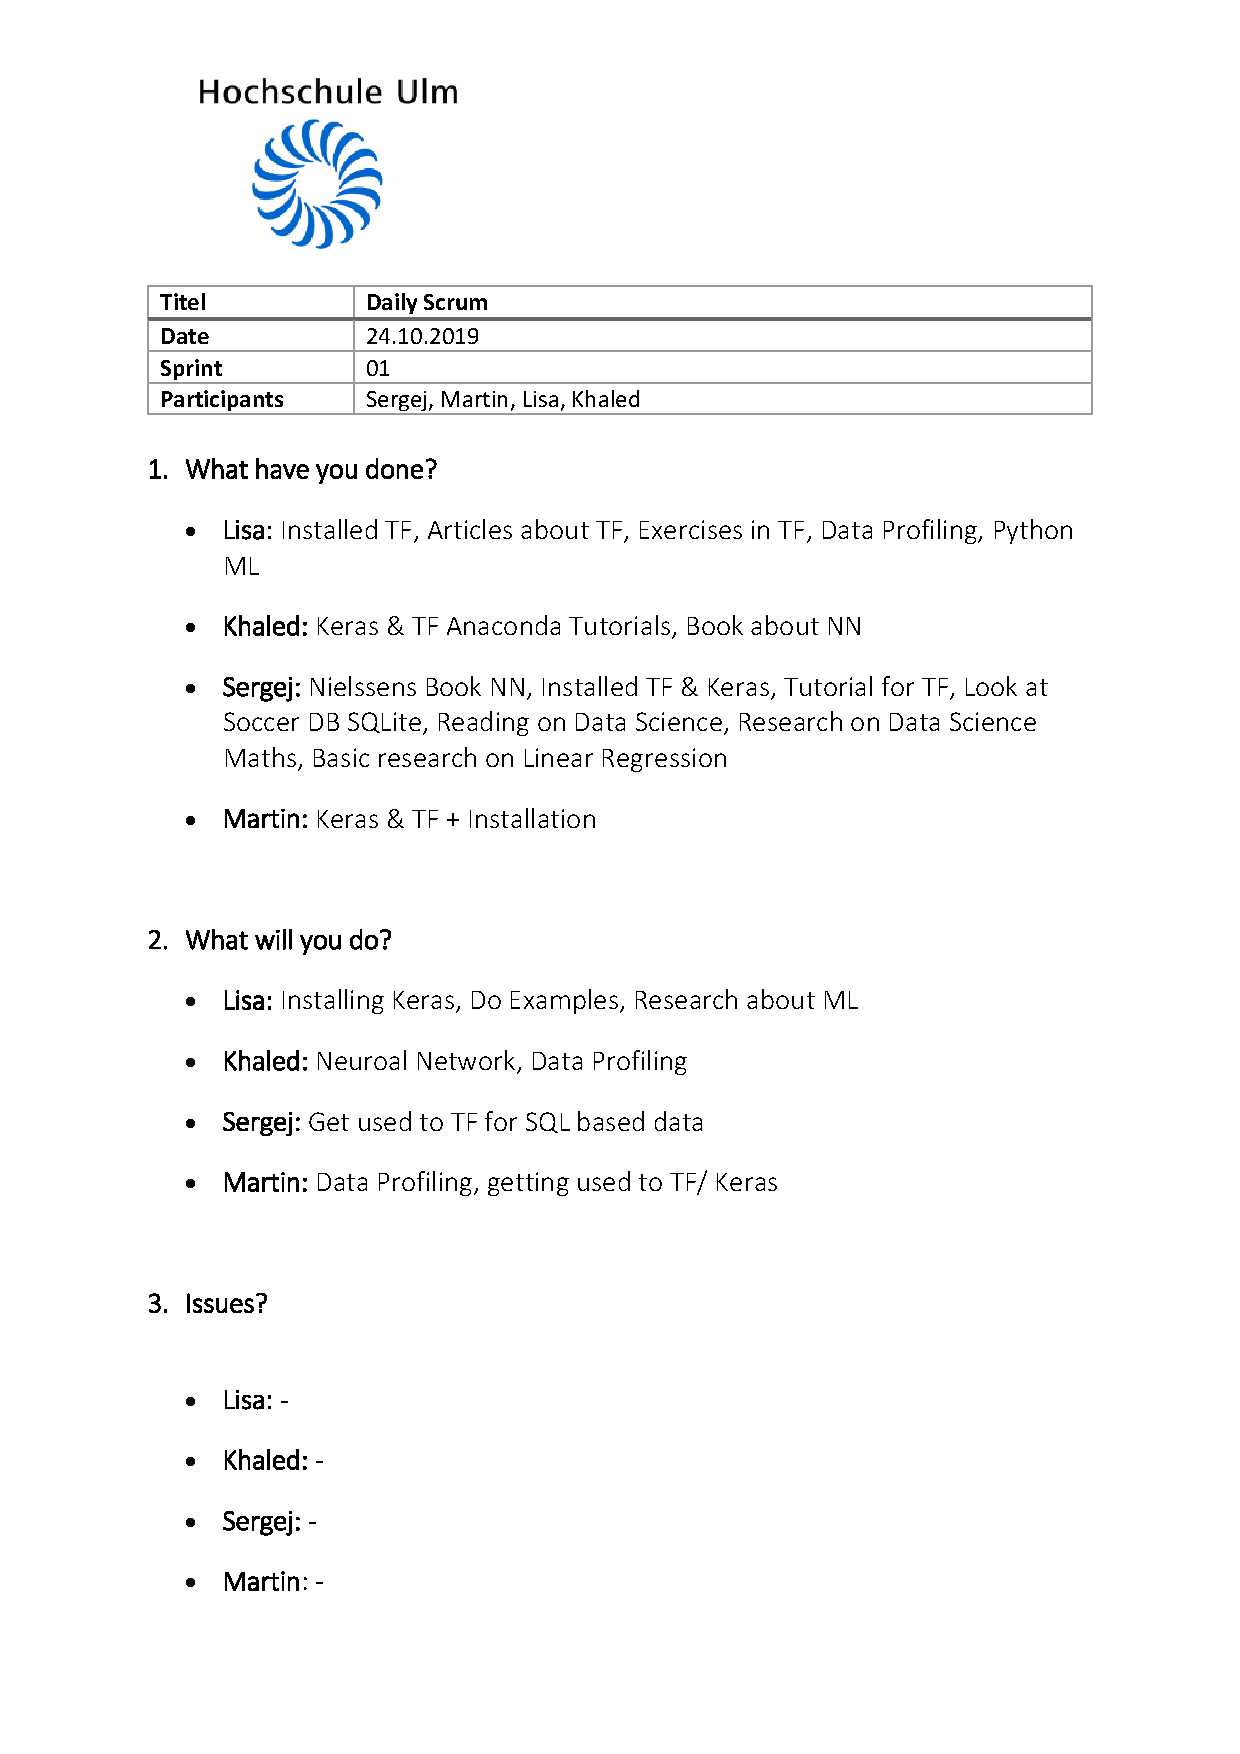
\includepdf[pages={1-2}]{pdf/Daily_Scrum_S01_1.pdf}

\includepdf[pages={1-2}]{pdf/Daily_Scrum_S01_2.pdf}

\includepdf[pages={1-2}]{pdf/Daily_Scrum_S02_1.pdf}
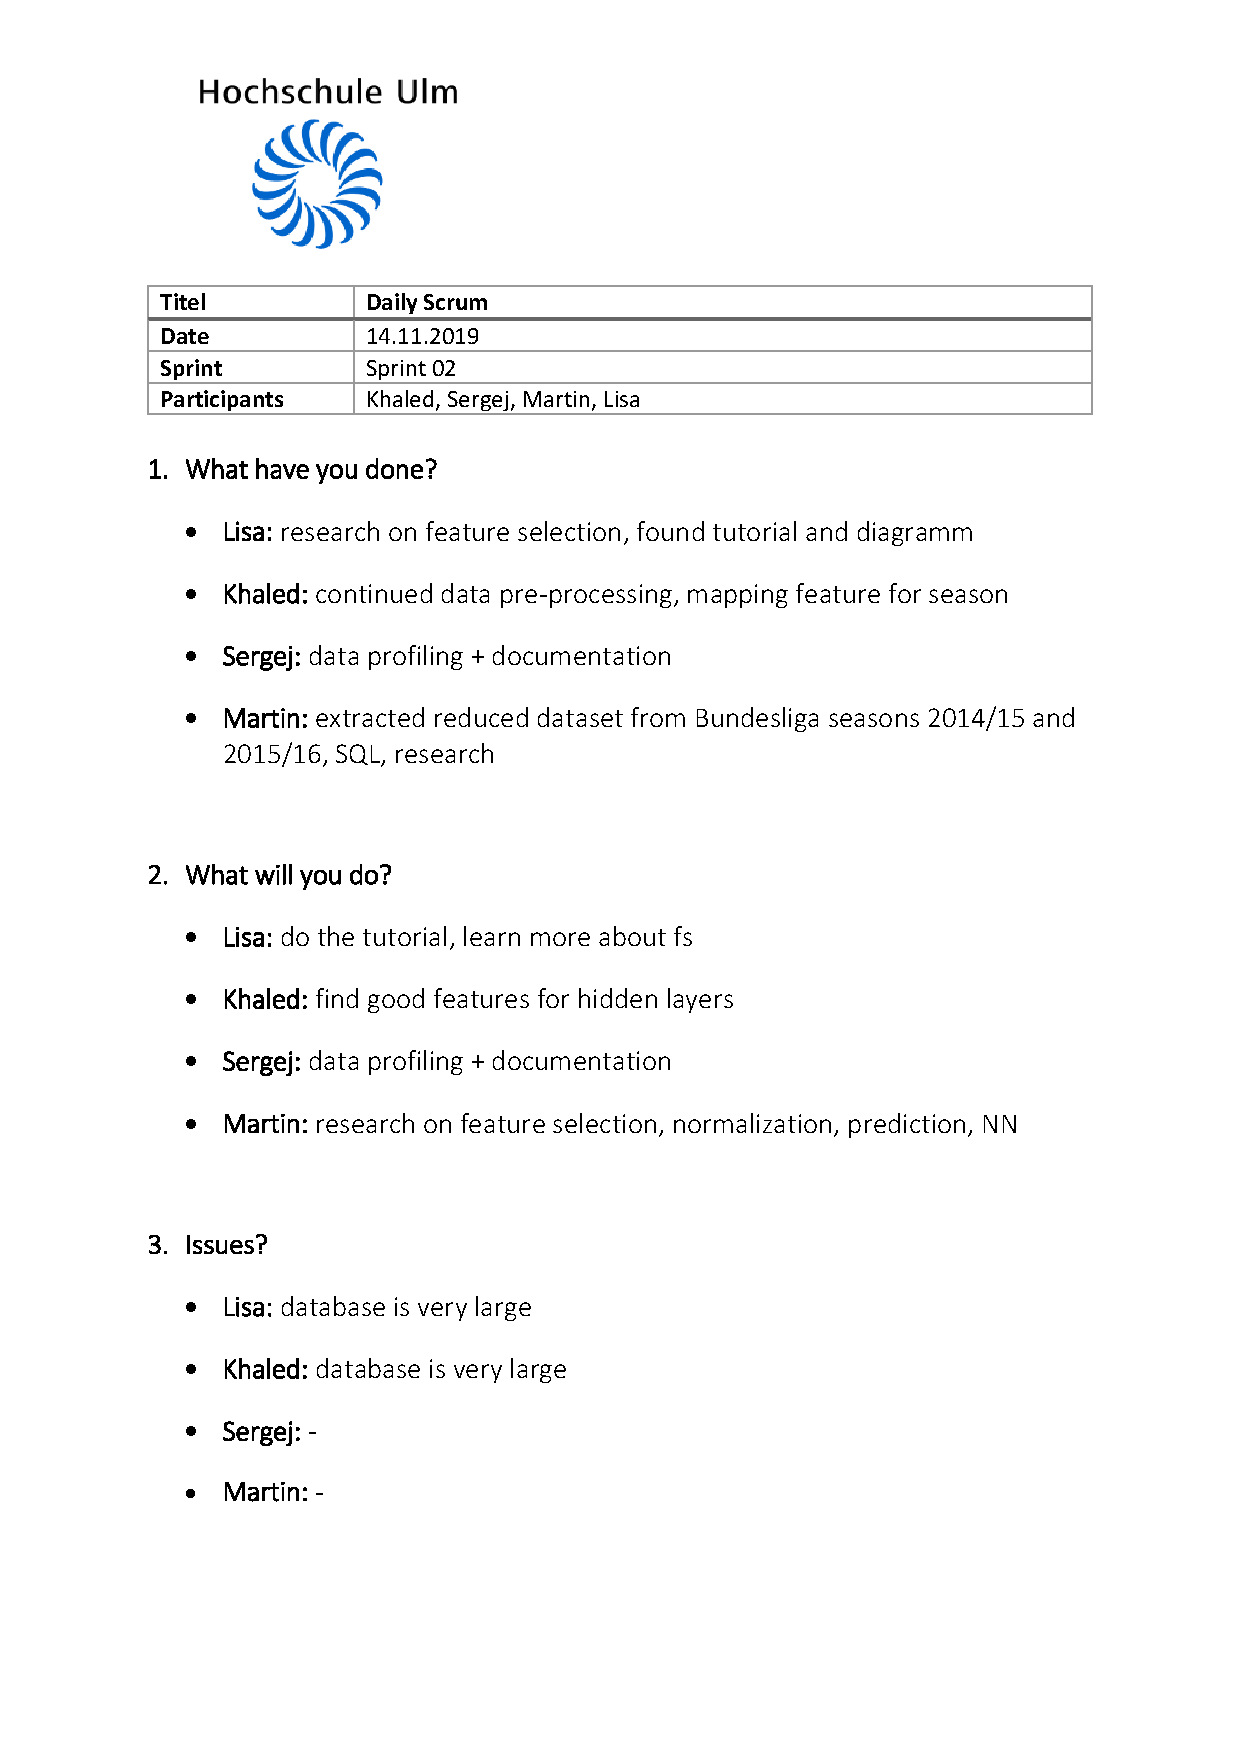
\includepdf[pages={1-2}]{pdf/Daily_Scrum_S02_2.pdf}
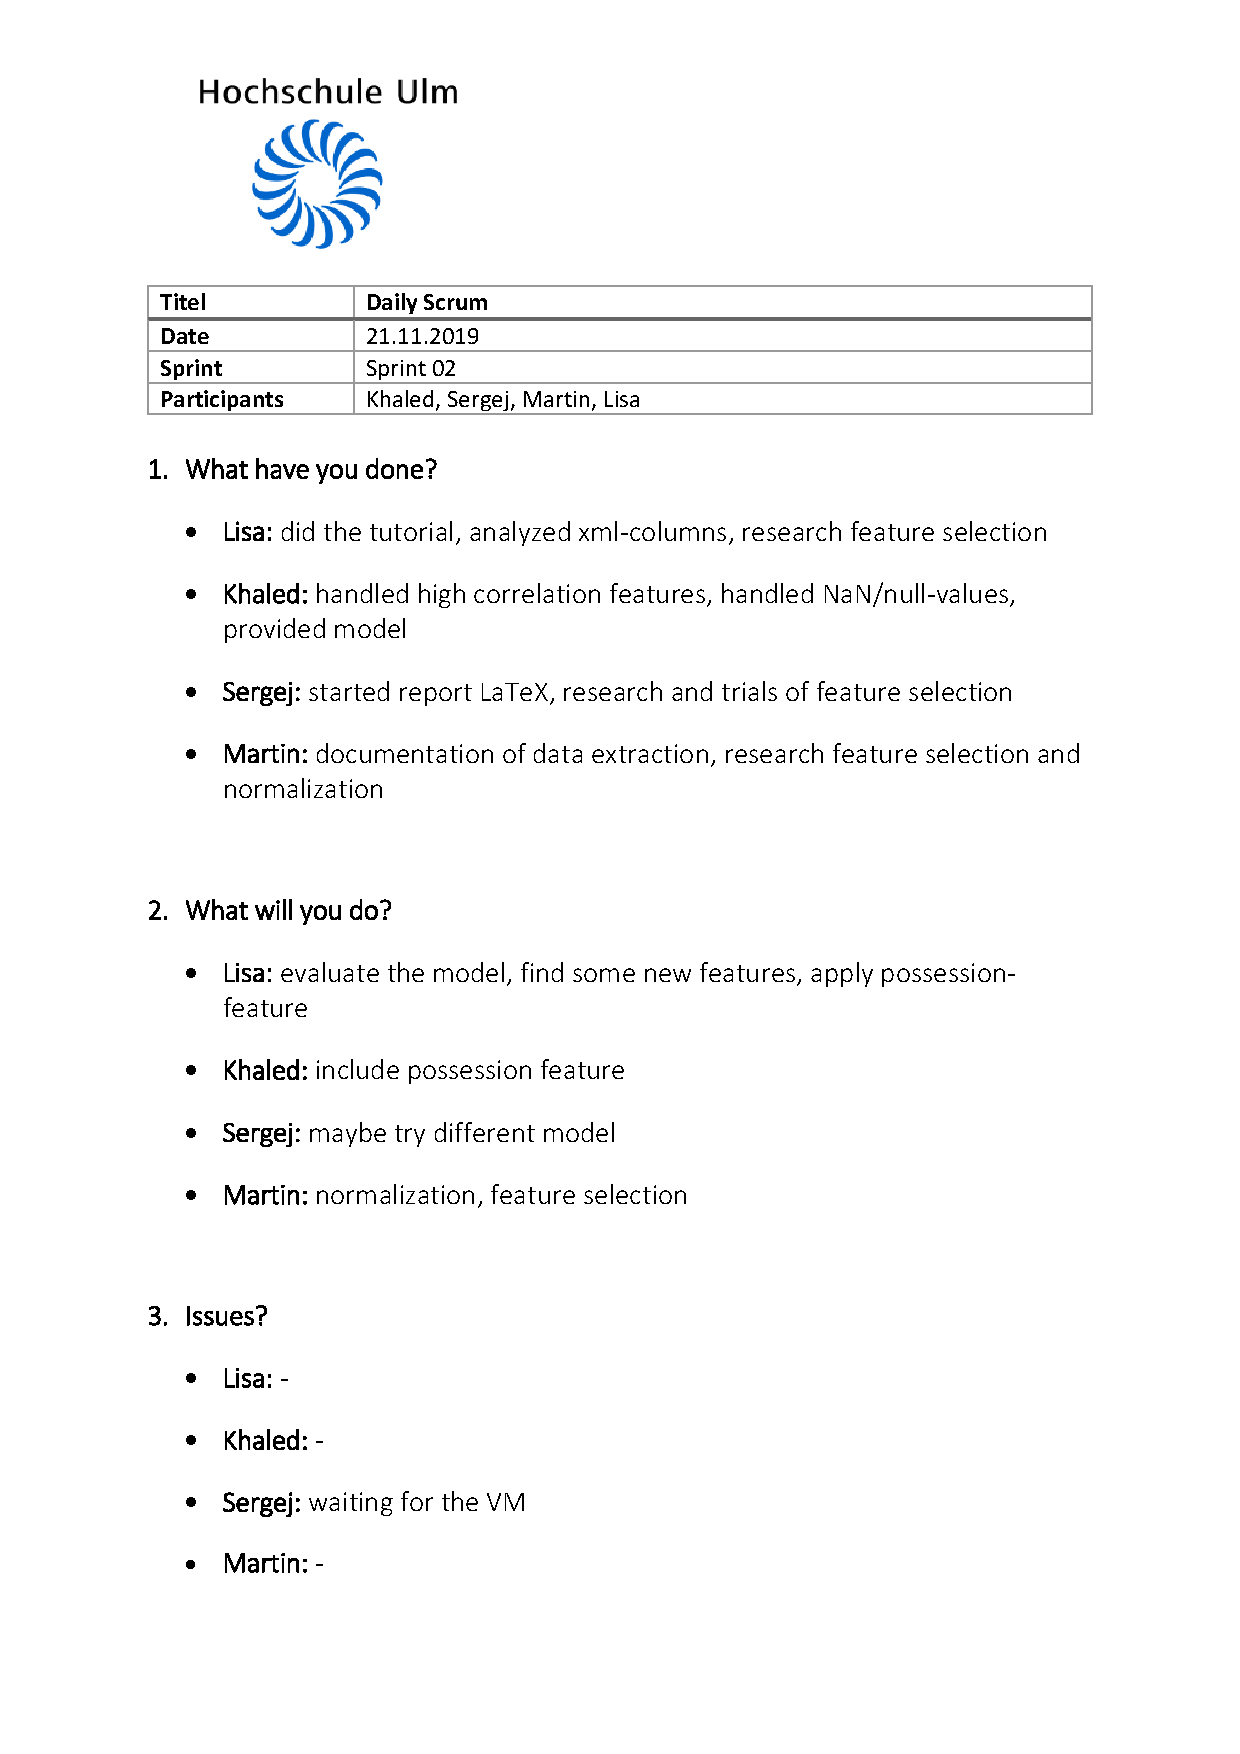
\includepdf[pages={1-2}]{pdf/Daily_Scrum_S02_3.pdf}
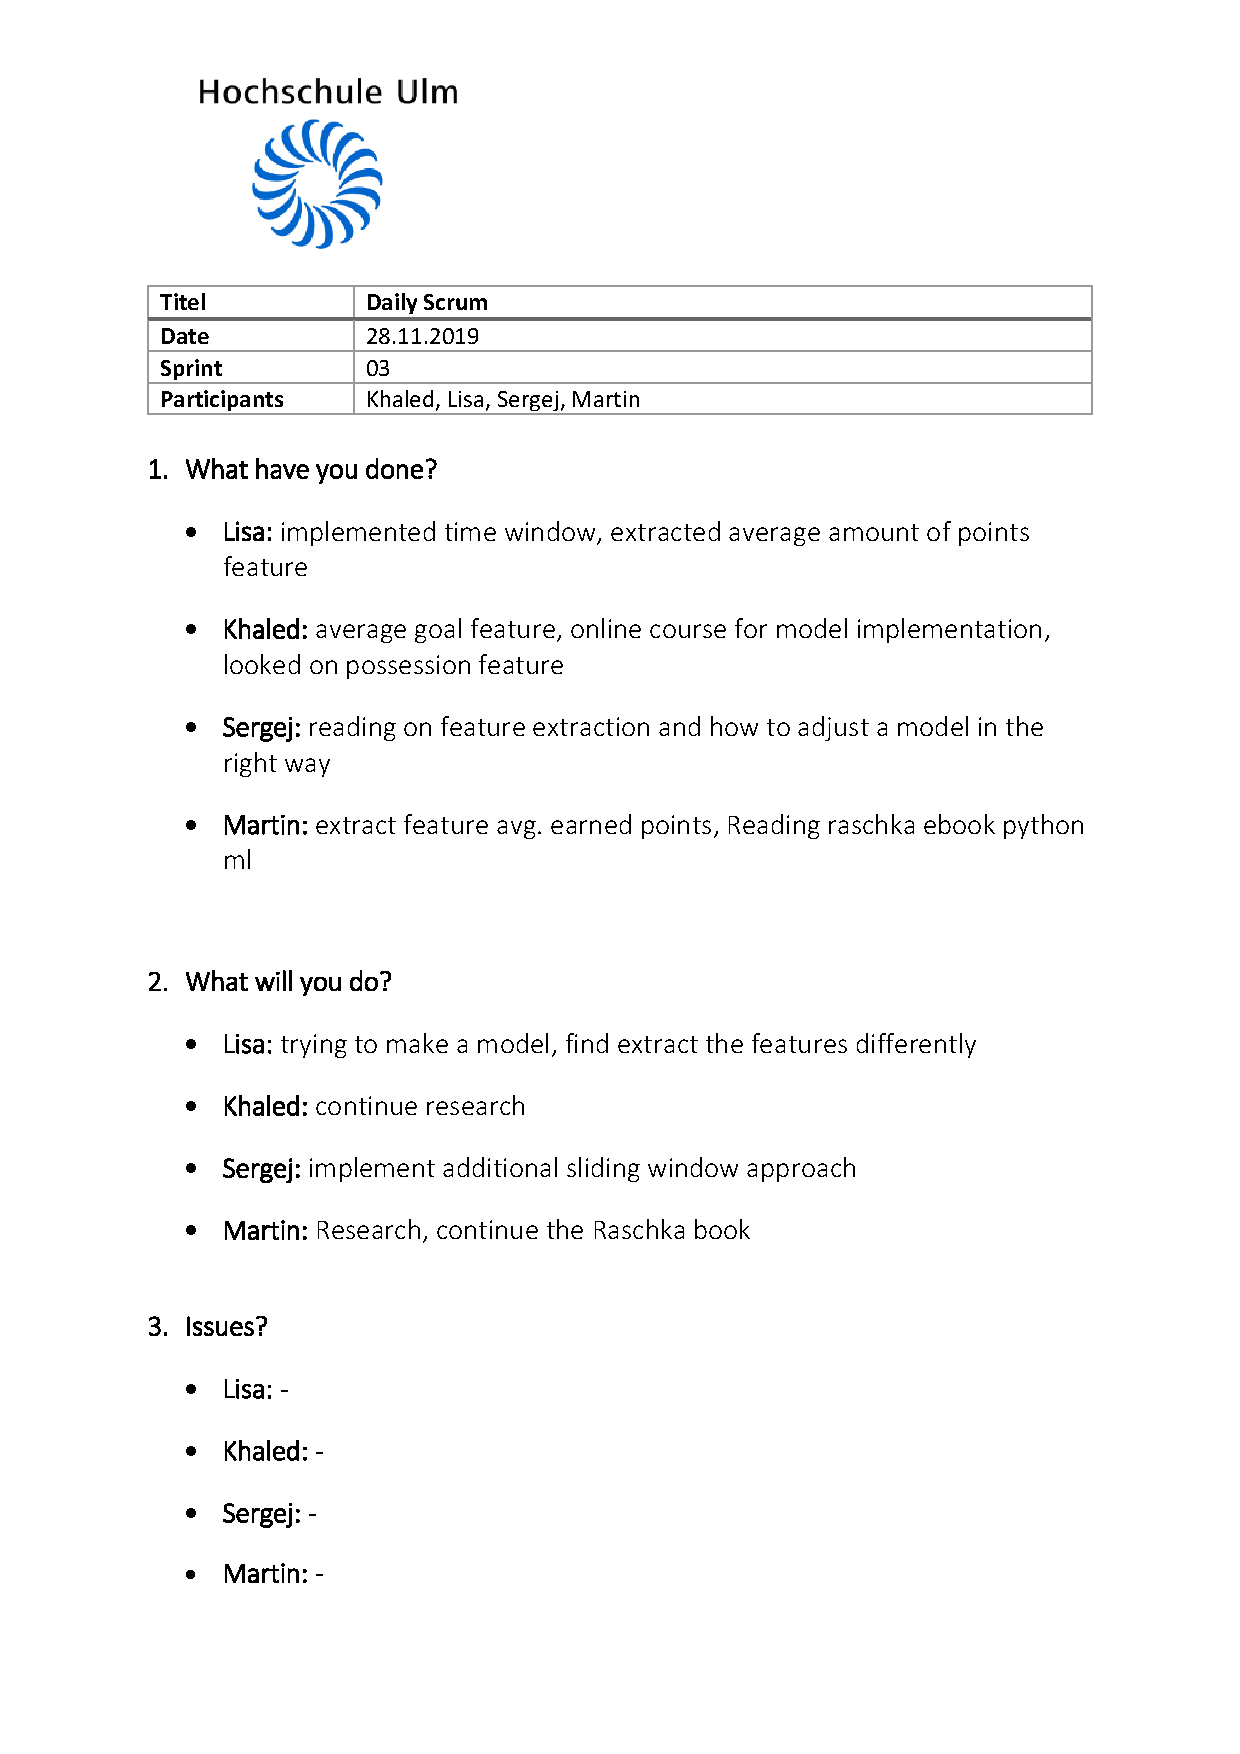
\includepdf[pages={1-2}]{pdf/Daily_Scrum_S03_1.pdf}
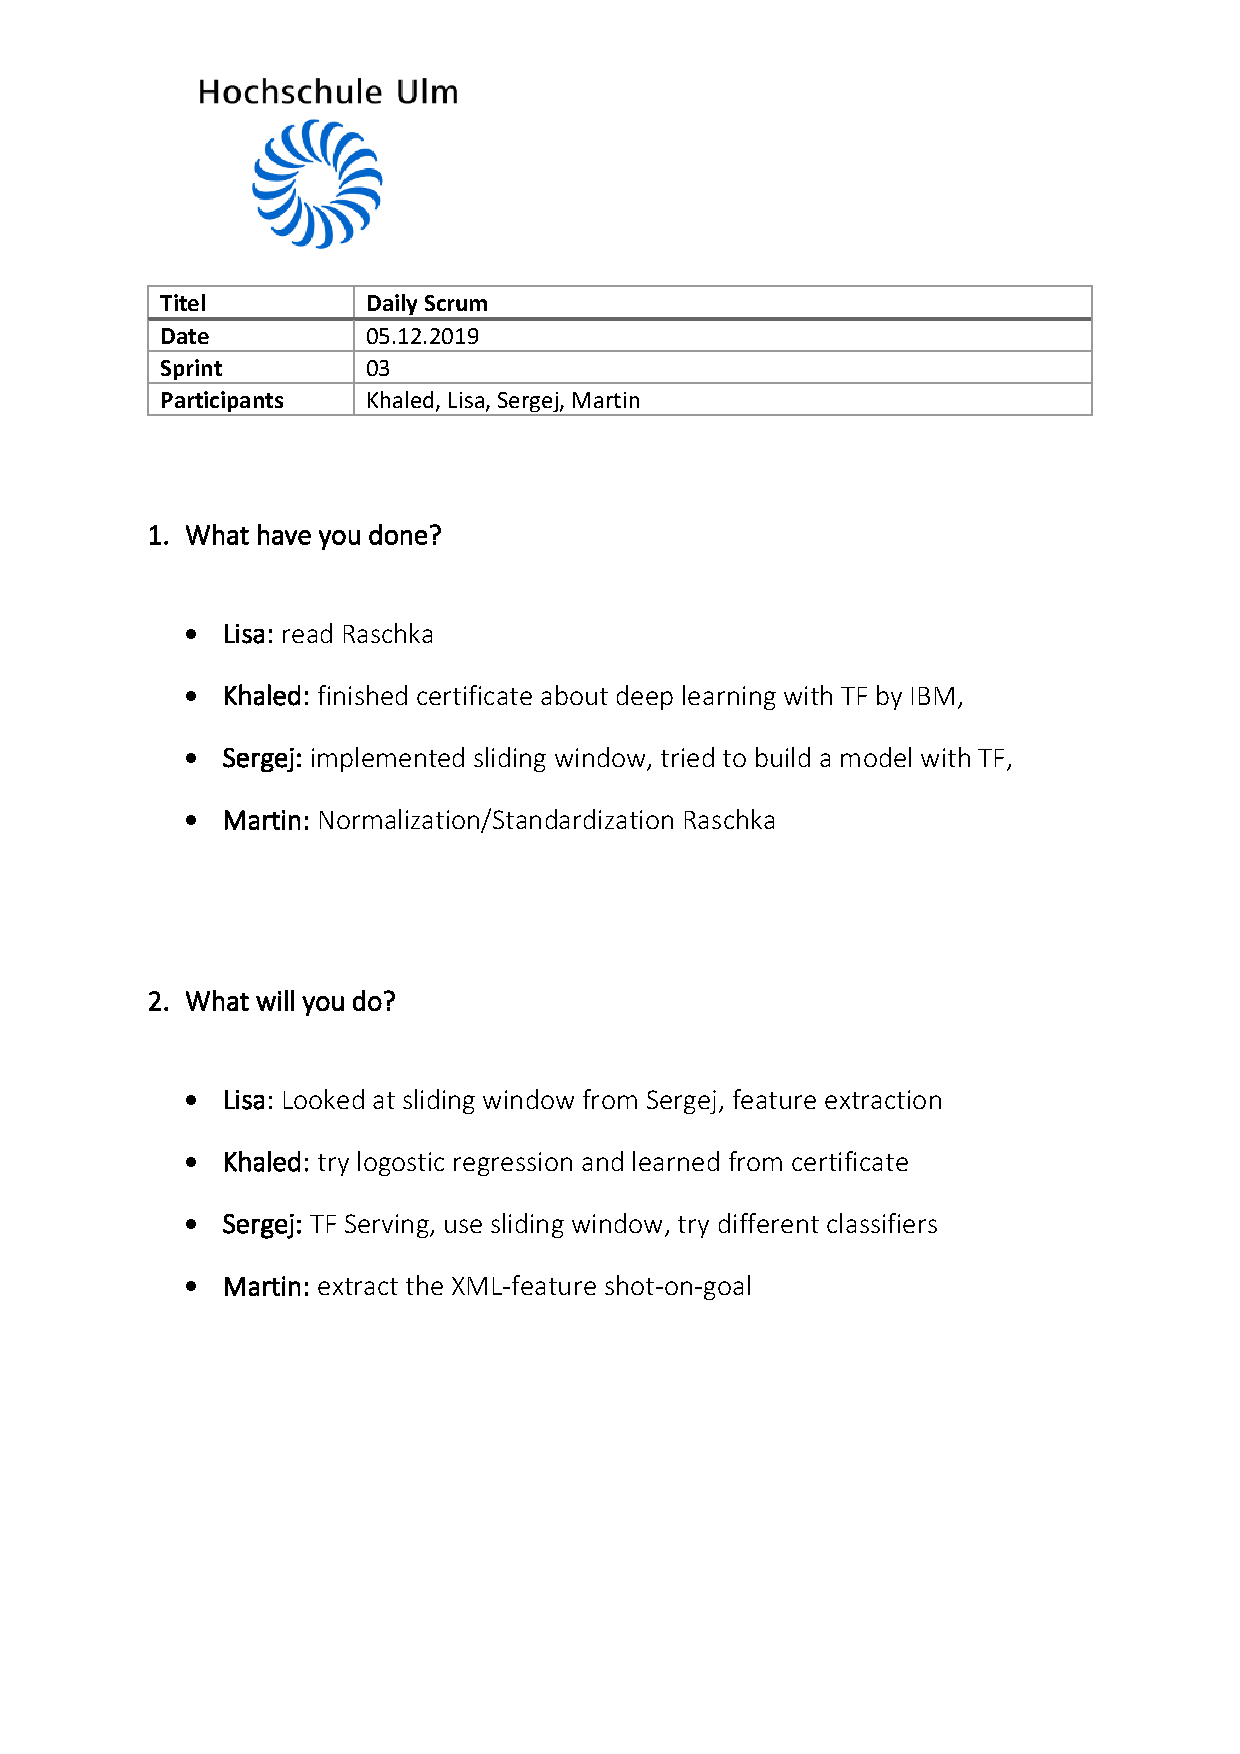
\includepdf[pages={1-2}]{pdf/Daily_Scrum_S03_2.pdf}
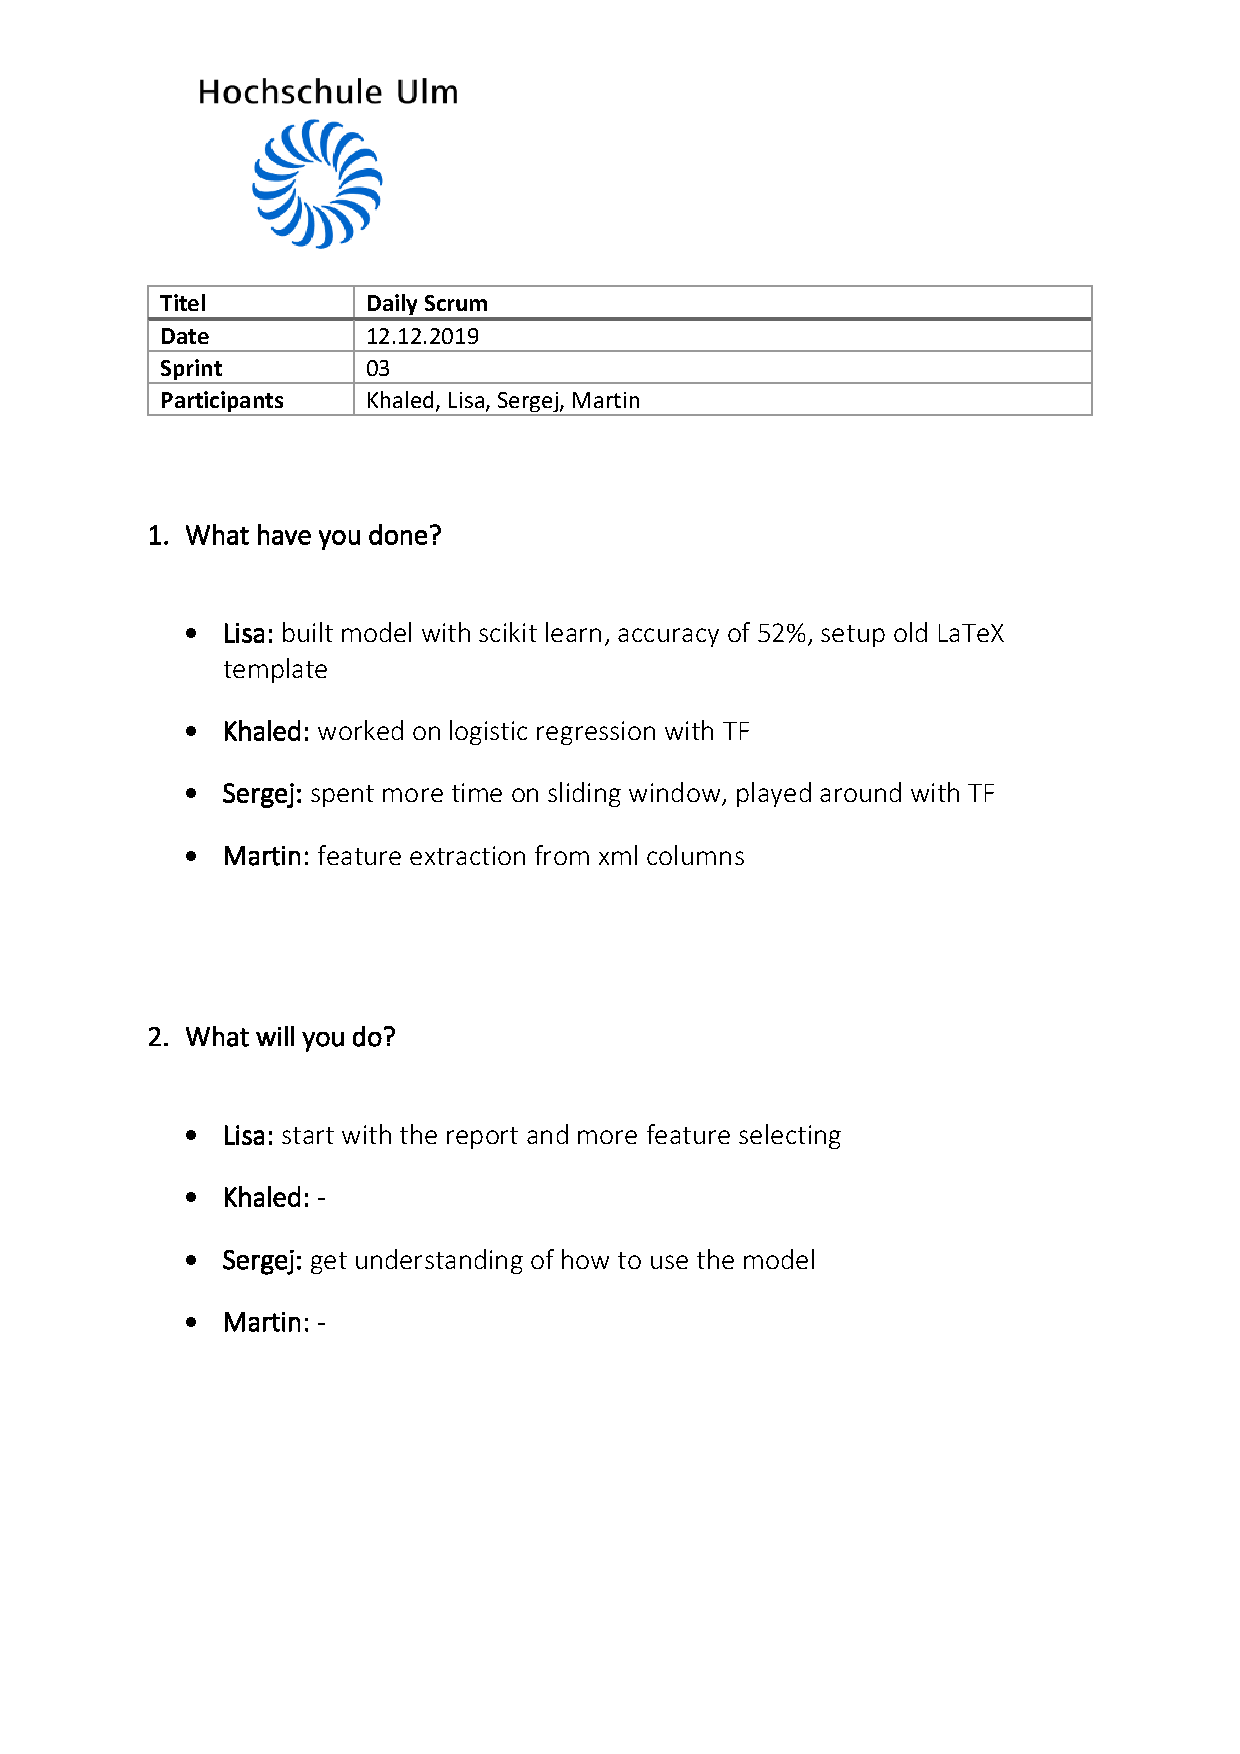
\includepdf[pages={1-2}]{pdf/Daily_Scrum_S03_3.pdf}
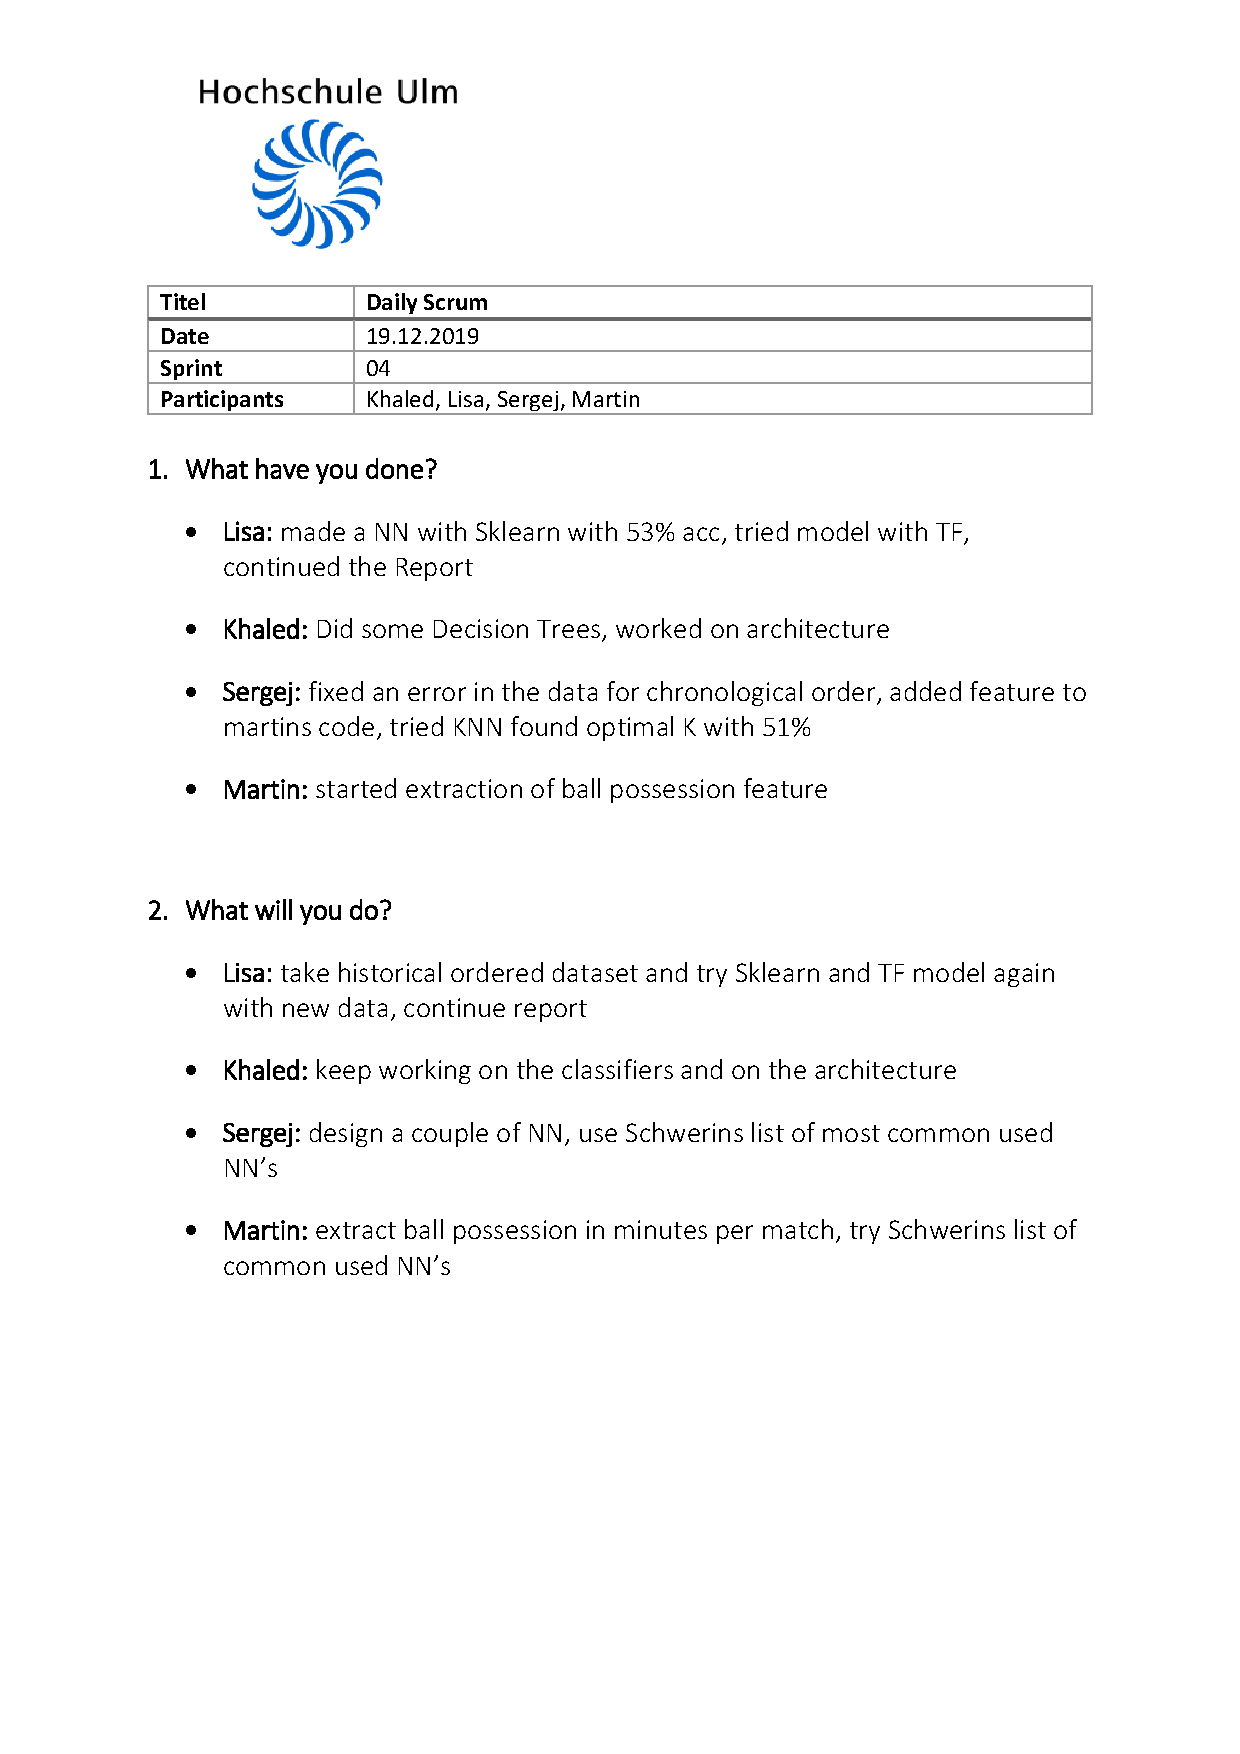
\includepdf[pages={1-2}]{pdf/Daily_Scrum_S04_1.pdf}
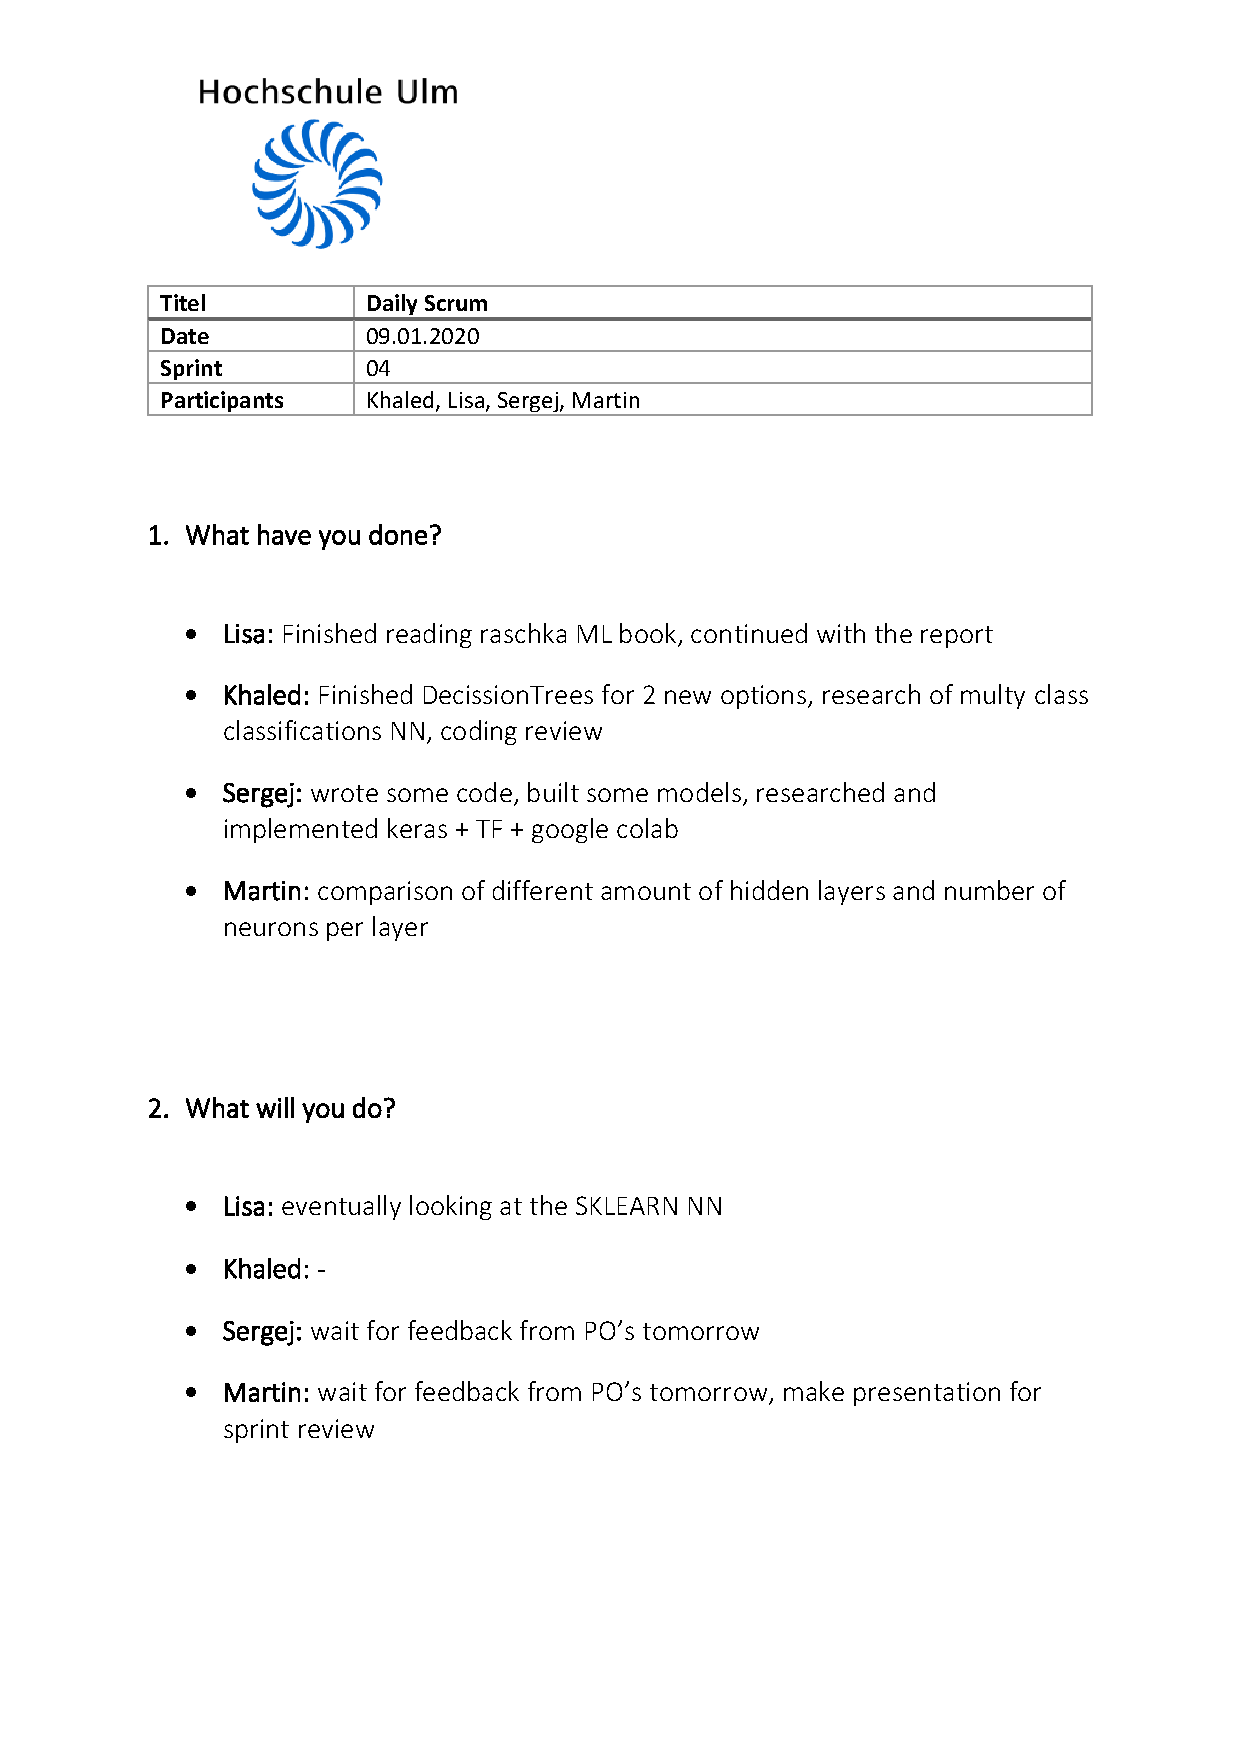
\includepdf[pages={1-2}]{pdf/Daily_Scrum_S04_2.pdf}

\newpage
\section{ Report of First Semester}
\label{section:appendix_c}
\newpage
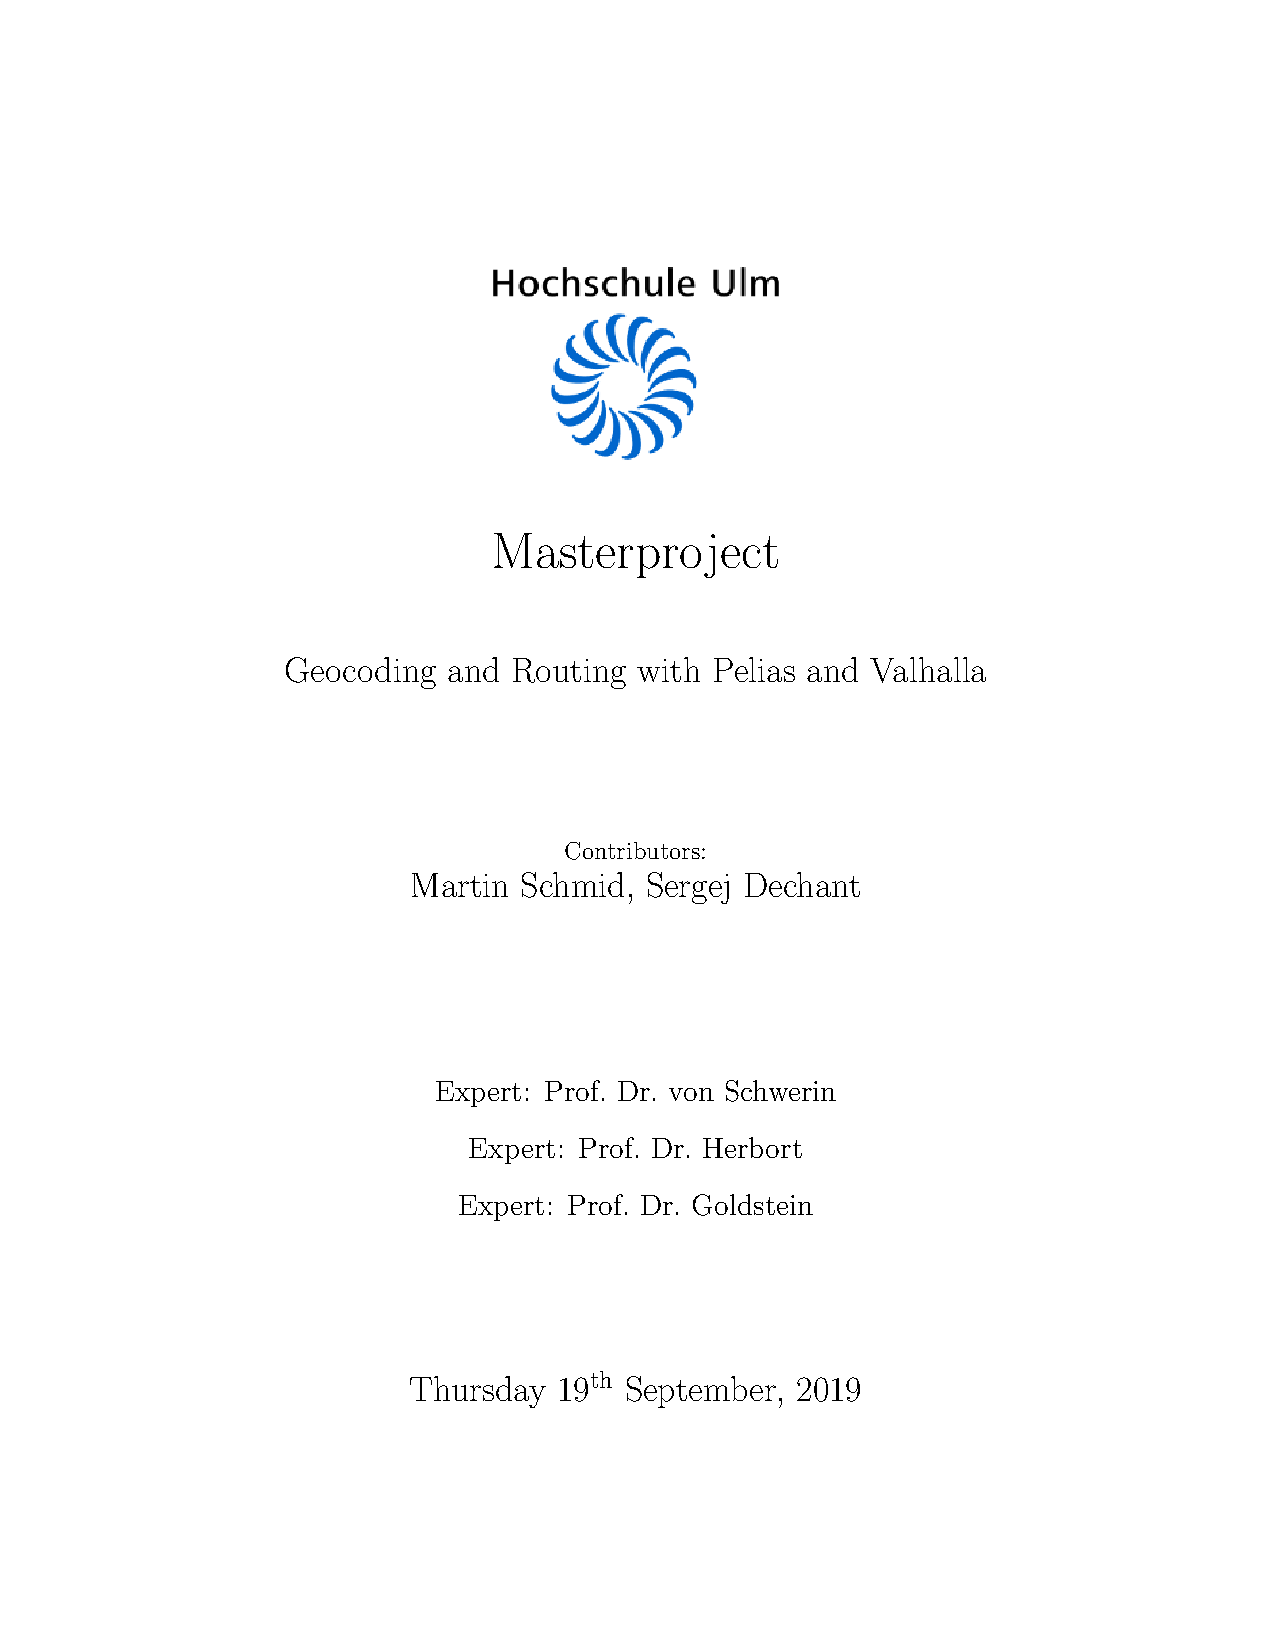
\includepdf[pages={1-30}]{pdf/ReportSemester1.pdf}
